\section{Evaluation}

\subsection{Method}

The evaluation combined ten functional scenarios and six non-functional scenarios.
Functional tests covered acquisition from all three source categories, offline persistence, offline batch creation, display of batch status, provenance preservation, access grant, authorized listing and reading, tampering rejection, and revocation.
Non-functional tests targeted authorization (NF01), confidentiality (NF02), integrity (NF03), provenance completeness (NF04), workload capacity (NF05), and temporary-failure recovery (NF06).

The capacity test generated 151,200 valid synthetic records.
This represents 15 streams sampled once per minute for seven days:
\(15 \times 7 \times 24 \times 60 = 151{,}200\).
The test generator produced 600 records per second to create the backlog within a practical test duration.
A separate server-side test concurrently submitted 20 batches from 20 distinct patient accounts.
These workloads test loss, application stability, and per-patient object contention; they do not establish a production throughput or latency service-level agreement.

\subsection{Results}

All ten functional scenarios completed successfully.
The application retained records while offline, formed and later transmitted batches, displayed their state, and enabled an authorized clinician to retrieve, verify, decrypt, and inspect provenance.
After revocation, subsequent reads were denied before ciphertext or key-opening material was returned.
\mbox{Fig.~\ref{fig:capacity-results} and Table~\ref{tab:nf-results}} summarize the capacity, security, and operational results.

All 151,200 generated records were processed without loss or application failure.
All 20 concurrently submitted batches were accepted, with zero failed submissions.

\begin{figure}[t]
	\centering
	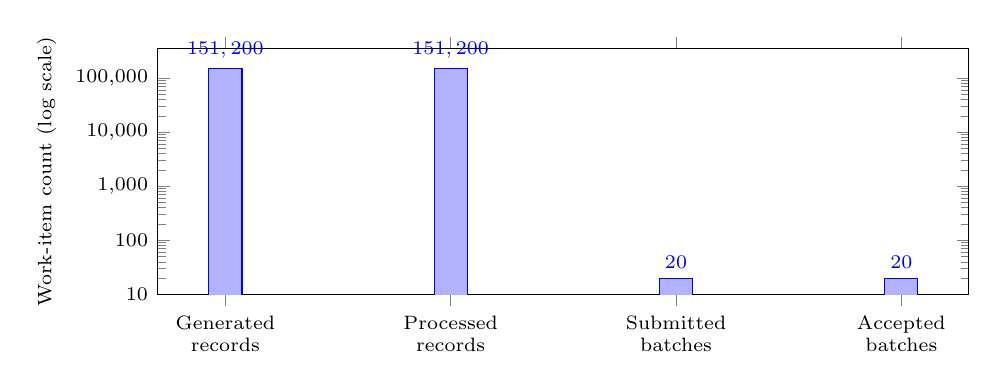
\begin{tikzpicture}
		\begin{axis}[
				ybar,
				ymode=log,
				log ticks with fixed point,
				width=0.98\columnwidth,
				height=4.7cm,
				ymin=10,
				ymax=350000,
				ytick={10,100,1000,10000,100000},
				xtick={1,2,3,4},
				xticklabels={{Generated\\records},{Processed\\records},{Submitted\\batches},{Accepted\\batches}},
				x tick label style={font=\scriptsize,align=center},
				y tick label style={font=\scriptsize},
				label style={font=\scriptsize},
				nodes near coords,
				point meta=rawy,
				nodes near coords style={font=\scriptsize,/pgf/number format/fixed,/pgf/number format/1000 sep={,}},
				bar width=12pt,
				ylabel={Work-item count (log scale)},
				fill=black!35,
				draw=black
			]
			\addplot coordinates {(1,151200) (2,151200) (3,20) (4,20)};
		\end{axis}
	\end{tikzpicture}
	\caption{Capacity-test outcomes. Generated/processed items are records; submitted/accepted items are batches.}
	\label{fig:capacity-results}
\end{figure}

Unauthorized requests with a missing or invalid token, or without an active \texttt{READ\_PGHD} capability, were rejected.
Inspection of PRE-bound payloads, IPFS objects, public IOTA metadata, denied responses, and relevant logs found no intelligible PGHD.
Changes to ciphertext, the recorded hash, signature, CID, IOTA metadata, or validity status were detected and rejected before the entry was treated as valid.
All required provenance fields were present for every tested source category.

\begin{table}[t]
	\caption{Non-Functional Evaluation}
	\label{tab:nf-results}
	\centering
	\scriptsize
	\begin{tabular}{@{}p{0.19\columnwidth}p{0.59\columnwidth}p{0.10\columnwidth}@{}}
		\toprule
		\shortstack[l]{\textbf{Test/}\\\textbf{property}} & \textbf{Observed evidence} & \textbf{Result} \\
		\midrule
		\textbf{NF01}\\Authorization & Missing, invalid, out-of-scope, expired, or revoked access returned neither PGHD nor key-opening material. & Pass \\
		\textbf{NF02}\\Confidentiality & No intelligible PGHD was found in inspected transit, IPFS, IOTA, denied responses, or logs. & Pass \\
		\textbf{NF03}\\Integrity & Changes to ciphertext, hash, signature, CID, metadata, and validity were detected and rejected. & Pass \\
		\textbf{NF04}\\Provenance & Patient, time, source, device/application, method, processing history, and validity were present. & Pass \\
		\textbf{NF05}\\Capacity & 151,200 records and 20 concurrent batches completed without loss or application failure. & Pass \\
		\textbf{NF06}\\Recovery & Unsent data persisted; after recovery, all tested units completed without observed duplication. & Pass \\
		\bottomrule
	\end{tabular}
\end{table}

During the recovery test, data remained locally available with a traceable failure state while connectivity or a supporting service was unavailable.
After service restoration, WorkManager retried the operation and every queued unit completed once in the tested run.
This result validates the implemented state and deduplication path for the injected failures, but it should not be generalized into a formal exactly-once guarantee across arbitrary distributed failures.

\FloatBarrier

\section{Discussion}

The results indicate that the architectural split is viable for DecMed.
Client-side encryption keeps PRE, IPFS, IOTA, and Redis outside the plaintext trust boundary.
The signed ciphertext hash lets both PRE and the clinician reject modifications, while the IPFS CID and IOTA state link stored content to an auditable metadata record.
PRE supports patient-controlled delegation without disclosing the patient's private key.
Finally, local persistence and batching decouple sensor collection from network and ledger availability.

Batching reduces remote operations but delays availability until a trigger fires.
Revocation blocks future key-material requests but cannot retract data already decrypted by a previously authorized clinician.
Provenance proves what the system recorded about origin and processing; it does not prove that a consumer wearable is clinically accurate.

The prototype was evaluated with one Android device, one wearable path, one PRE instance, a local IOTA/IPFS environment, and a desktop clinician client.
The 20-patient concurrency test was chosen to expose shared-object contention, not to model hospital-scale peak traffic.
The study does not report latency, energy consumption, ledger cost, long-duration reliability, or clinician usability.
Future work should evaluate asynchronous server queues, adaptive synchronization based on battery and network quality, larger multi-node deployments, credential recovery, interoperability with clinical data standards, and longitudinal use by patients and healthcare professionals.

\section{Conclusion}

This paper presented a PGHD module that extends DecMed from provider-generated records to patient-controlled, between-visit data.
The module combines offline-first local storage and batching with client-side AES-GCM encryption, SHA-256 and ECDSA integrity checks, PRE-based delegation, IPFS ciphertext storage, and IOTA-based access and validity metadata.
The prototype passed ten functional and six non-functional scenarios, processed 151,200 synthetic records without loss, and accepted 20 concurrent patient batches.
It also rejected the tested unauthorized and tampered requests and recovered queued data after temporary failures.
Within the stated prototype scope, the results support the feasibility of secure and traceable PGHD integration in DecMed.
